% =============================================================================
% Chapter 6: Complete Autonomous Navigation Algorithm
% Hebrew primary, English technical terms in \en{}
% XeLaTeX : requires \selectlanguage{hebrew} at top
% =============================================================================

\selectlanguage{hebrew}

\section{אלגוריתם ניווט אוטונומי מלא: מאקולוקציה לתכנון מסלול אדפטיבי}
\label{sec:ch06_algorithm}

\subsection{סקירת האלגוריתם המלא}
\label{sec:ch06_overview}

האלגוריתם המלא לניווט אוטונומי משלב את כל הרכיבים שהוצגו בפרקים הקודמים: מודל ביומימטי של אקולוקציה, עיבוד אותות אקוסטי, \en{SLAM} אקוסטי, מיזוג חיישנים רב-מודאלי, ותכנון מסלול אדפטיבי. האלגוריתם פועל בלולאה סגורה (\en{closed-loop}) בתדר 50 הרץ, כאשר בכל מחזור עיבוד מבוצעים השלבים הבאים: רכישת מדידות חיישנים, חיזוי מצב באמצעות \en{IMU}, עיבוד הדים אקוסטיים, עדכון מפת \en{SLAM}, מיזוג מדידות ב\en{EKF}, תכנון מסלול, ושליחת פקודות בקרה לרחפן. \cite{Thrun2005ProbRobotics} \cite{CrewAIDocs}

האלגוריתם מתוכנן לפעול בזמן אמת על פלטפורמת \en{NVIDIA Jetson Orin NX} עם מגבלות משאבים מחמירות. כל שלב באלגוריתם מחושב מראש מבחינת זמן ריצה וצריכת זיכרון, והמערכת כוללת מנגנון ניהול משאבים אדפטיבי המתאים את תצורת העיבוד בהתאם לעומס המעבד ולמצב הסוללה. \cite{CrewAIDocs}

\subsection{אלגוריתם ראשי: לולאת ניווט ראשית}
\label{sec:ch06_main_loop}

האלגוריתם הראשי מנוהל על ידי לולאת בקרה בתדר 50 הרץ. להלן הפסאודו-קוד של הלולאה הראשית:

\begin{english}
\begin{lstlisting}[language=Python, caption=לולאת ניווט ראשית - האלגוריתם המלא לניווט אוטונומי. (Main navigation loop - complete autonomous navigation algorithm.), label=lst:ch06_main_loop, basicstyle=\small\ttfamily, numbers=left, numberstyle=\tiny, frame=single, breaklines=true]
def navigation_loop():
    # אתחול מערכת
    x_0 = initialize_state()
    P_0 = initialize_covariance()
    map = initialize_occupancy_grid()
    path = initialize_path()
    
    k = 0
    while not mission_complete:
        # שלב 1: רכישת מדידות חיישנים
        imu_data = read_imu()           # 200 Hz
        sonar_data = read_sonar()       # 20 Hz
        optical_flow = read_optical()   # 30 Hz
        
        # שלב 2: חיזוי מצב באמצעות IMU
        x_pred, P_pred = $e$k$f_predict(x_k, P_k, imu_data)$$$
        
        # שלב 3: עיבוד הדים אקוסטיים
        if sonar_data.available:
            echoes = $m$a$tched_filter(sonar_data.raw)$$$
            echoes = mvdr_beamforming(echoes)
            features = cnn_classify(echoes)
            
        # שלב 4: עדכון מפת SLAM
        if sonar_data.available:
            map = $u$p$date_occupancy_grid(map, x_pred, echoes)$$$
            loop_candidate = detect_loop_closure(map, echoes)
            if loop_candidate is not None:
                map = $o$p$timize_pose_graph(map, loop_candidate)$$$
                
        # שלב 5: מיזוג מדידות ב-EKF
        if sonar_data.available:
            x_k, P_k = $e$k$f_update_sonar(x_pred, P_pred, echoes)$$$
        elif optical_flow.available:
            x_k, P_k = $e$k$f_update_optical(x_pred, P_pred, optical_flow)$$$
        else:
            x_k, P_k = x_pred, P_pred
            
        # שלב 6: תכנון מסלול אדפטיבי
        if k % planning_interval == 0:
            path = $a$d$aptive_rrt_star(x_k, map, P_k)$$$
            
        # שלב 7: שליחת פקודות בקרה
        control = $c$o$mpute_control(x_k, path)$$$
        send_control(control)
        
        # שלב 8: ניהול משאבים אדפטיבי
        if k % resource_interval == 0:
            $a$d$just_processing_mode(battery, cpu_load)$$$
            
        k = k + 1
        $s$l$eep(1.0 / CONTROL_FREQUENCY)$$$
\end{lstlisting}
\end{english}

האלגוריתם מבצע 8 שלבים בכל מחזור עיבוד. זמן הריצה הכולל של מחזור עיבוד מלא הוא כ-24.1 אלפיות-שנייה, מתוך תקציב של 50 אלפיות-שנייה. שאר הזמן משמש להמתנה למדידה הבאה ולטיפול במשימות רקע. \cite{CrewAIDocs}

\subsection{אלגוריתם תכנון מסלול RRT* אדפטיבי}
\label{sec:ch06_rrt_star}

מתכנן המסלול מבוסס \en{RRT*} (\en{Rapidly-exploring Random Tree Star}) מותאם לאי-ודאות חישה משתנה. האלגוריתם בונה עץ של מסלולים אפשריים מהמיקום הנוכחי ליעד, תוך התחשבות במכשולים, באי-ודאות המיקום, ובאיכות החישה. פונקציית העלות של מסלול $\tau$ היא: \cite{Thrun2005ProbRobotics}

\begin{equation}
J(\tau) = w_1 \cdot \text{length}(\tau) + w_2 \cdot \text{risk}(\tau) + w_3 \cdot \text{energy}(\tau)
\label{eq:ch06_cost_function}
\end{equation}

כאשר $\text{length}(\tau)$ הוא אורך המסלול, $\text{risk}(\tau)$ הוא סיכון ההתנגשות (מבוסס על אי-ודאות המיקום וקרבה למכשולים), $\text{energy}(\tau)$ היא צריכת האנרגיה המשוערת, ו-$w_1, w_2, w_3$ הם משקלים הניתנים לכיול. \cite{CrewAIDocs}

אופק החישה האדפטיבי (\en{adaptive sensing horizon}) מותאם למרחק למכשול הקרוב ולאיכות ההדים:

\begin{equation}
R_{\text{max}} = \min\l$e$f$t( R_{\text{nominal}}, \frac{\text{SNR}}{\text{SNR}_{\text{threshold}}} \cdot R_{\text{nominal}} \right)$$$
\label{eq:ch06_adaptive_horizon}
\end{equation}

כאשר $R_{\text{nominal}} = 15$ מטר הוא הטווח הנומינלי, $\text{SNR}$ הוא יחס האות לרעש הנוכחי, ו-$\text{SNR}_{\text{threshold}} = 10$ dB הוא סף יחס האות לרעש המינימלי. \cite{CrewAIDocs}

\subsection{אלגוריתם זיהוי לולאות סגירה אקוסטיות}
\label{sec:ch06_loop_closure_algo}

זיהוי לולאות סגירה מתבצע באמצעות השוואת מפת ההדים הנוכחית למפות קודמות. האלגוריתם משתמש במטריצת \en{ScanContext} אקוסטית ובאימות גאומטרי באמצעות \en{ICP}. להלן הפסאודו-קוד של האלגוריתם:

\begin{english}
\begin{lstlisting}[language=Python, caption=אלגוריתם זיהוי לולאות סגירה אקוסטיות. (Acoustic loop closure detection algorithm.), label=lst:ch06_loop_closure, basicstyle=\small\ttfamily, numbers=left, numberstyle=\tiny, frame=single, breaklines=true]
def $d$e$tect_loop_closure(map, current_echoes)$$$:
    # בניית מטריצת ScanContext אקוסטית
    SC_current = $b$u$ild_scan_context(current_echoes)$$$
    
    # חיפוש במסד הנתונים של ScanContexts קודמים
    best_match = None
    best_distance = float('inf')
    
    for SC_prev in database:
        # חישוב מרחק בין ScanContexts
        distance = $s$c$an_context_distance(SC_current, SC_prev)$$$
        
        if distance < LOOP_CLOSURE_THRESHOLD:
            # אימות גאומטרי באמצעות ICP
            T_icp, inliers = $i$c$p_registration(
                current_echoes, 
                database.get_echoes(SC_prev)$$$
            )
            
            if inliers > MIN_INLIERS:
                if distance < best_distance:
                    best_distance = distance
                    best_match = (SC_prev, T_icp)
    
    # הוספת ScanContext נוכחי למסד הנתונים
    database.$a$p$pend(SC_current)$$$
    
    return best_match
\end{lstlisting}
\end{english}

האלגוריתם משיג שיעור הצלחה של 87\% בזיהוי לולאות סגירה במנהרה ו-72\% במחסן. השימוש ב\en{GNN} להתאמת הדים משפר את שיעור הזיהוי ב-15\% לעומת שיטות התאמה מסורתיות מבוססות טווח-אזימוט בלבד. \cite{CrewAIDocs}

\subsection{אלגוריתם מיזוג EKF אדפטיבי}
\label{sec:ch06_adaptive_ekf}

אלגוריתם מיזוג ה\en{EKF} האדפטיבי משלב את שלב החיזוי מבוסס \en{IMU} עם עדכונים מהחיישן העל-קולי ומחיישן הזרימה האופטית. האלגוריתם כולל מנגנון אומדן קווריאנס אדפטיבי המזהה השפלת חיישן ומתאים את משקלו באומדן המצב. להלן הפסאודו-קוד:

\begin{english}
\begin{lstlisting}[language=Python, caption=אלגוריתם מיזוג EKF אדפטיבי עם זיהוי השפלת חיישן. (Adaptive EKF fusion algorithm with sensor degradation detection.), label=lst:ch06_adaptive_ekf, basicstyle=\small\ttfamily, numbers=left, numberstyle=\tiny, frame=single, breaklines=true]
def $a$d$aptive_ekf_fusion(x_pred, P_pred, measurements)$$$:
    x = x_pred
    P = P_pred
    
    # עדכון מחיישן על-קולי
    if 'sonar' in measurements:
        z_sonar = measurements['sonar']
        H_sonar = compute_jacobian_sonar(x)
        R_sonar = get_adaptive_R('sonar')
        
        # מבחן כי-ריבוע לזיהוי השפלה
        innovation = z_sonar - h_sonar(x)
        S = H_sonar @ P @ H_sonar.T + R_sonar
        mahalanobis = innovation.T @ np.linalg.inv(S) @ innovation
        
        if mahalanobis > CHI2_THRESHOLD:
            # השפלה: הגדלת קווריאנס רעש המדידה
            R_sonar = R_sonar * DEGRADATION_FACTOR
            $u$p$date_adaptive_R('sonar', R_sonar)$$$
        
        # עדכון EKF סטנדרטי
        K = P @ H_sonar.T @ np.linalg.inv(S)
        x = x + K @ innovation
        P = (np.eye(len(x)) - K @ H_sonar) @ P
    
    # עדכון מחיישן זרימה אופטית
    if 'optical_flow' in measurements:
        z_flow = measurements['optical_flow']
        H_flow = compute_jacobian_flow(x)
        R_flow = $g$e$t_adaptive_R('optical_flow')$$$
        
        innovation = z_flow - h_flow(x)
        S = H_flow @ P @ H_flow.T + R_flow
        
        K = P @ H_flow.T @ np.linalg.inv(S)
        x = x + K @ innovation
        P = (np.eye(len(x)) - K @ H_flow) @ P
    
    return x, P
\end{lstlisting}
\end{english}

האלגוריתם מזהה השפלת חיישן תוך 200 אלפיות-שנייה ומתאים את משקל החיישן באומדן המצב בהתאם. מנגנון זה קריטי לשמירה על יציבות המערכת בתנאי הפעלה משתנים, כגון מעבר מסביבה מוארת לחשוכה או כניסה לעשן. \cite{Thrun2005ProbRobotics} \cite{CrewAIDocs}

\subsection{אלגוריתם ניהול משאבים אדפטיבי}
\label{sec:ch06_resource_management}

מערכת ניהול המשאבים האדפטיבית מתאימה את תצורת העיבוד בהתאם למצב הסוללה, עומס המעבד, ואיכות החישה. המערכת פועלת בשלושה מצבים: ביצועים גבוהים, בינוני, וחיסכון. המעבר בין המצבים מבוסס על פונקציית החלטה המשלבת את כל הגורמים: \cite{CrewAIDocs}

\begin{equation}
M = \begin{cases}
\text{high} & \text{אם } B > 50\% \text{ ו-} L < 60\% \\
\text{medium} & \text{אם } 20\% < B \leq 50\% \text{ או } 60\% \leq L < 80\% \\
\text{low} & \text{אם } B \leq 20\% \text{ או } L \geq 80\%
\end{cases}
\label{eq:ch06_mode_selection}
\end{equation}

כאשר $B$ הוא מצב הסוללה באחוזים ו-$L$ הוא עומס המעבד באחוזים. במצב חיסכון, תדר העיבוד האקוסטי מופחת ל-10 הרץ, עיבוד ה\en{SLAM} מופחת ל-1 הרץ, ותכנון המסלול מושבת (מעבר לניווט תגובתי בלבד). במצב זה, צריכת ההספק הכוללת יורדת מ-15 וואט ל-8 וואט, ומשך המשימה גדל מ-18 דקות ל-32 דקות. \cite{CrewAIDocs}

\subsection{אלגוריתם הימנעות ממכשולים עם אופק חישה אדפטיבי}
\label{sec:ch06_obstacle_avoidance}

אלגוריתם ההימנעות ממכשולים משלב את מתכנן המסלול \en{RRT*} עם פונקציית עונש קרבה למכשול (\en{Control Barrier Function, CBF}) המבטיחה שהרחפן לא יתקרב למכשול מעבר למרחק בטוח. פונקציית העונש מוגדרת כ: \cite{Thrun2005ProbRobotics}

\begin{equation}
\Phi(\mathbf{x}) = \sum_{i} \max\l$e$f$t(0, 1 - \frac{\|\mathbf{x} - \mathbf{m}_i\|}{d_{\text{safe}}}\right)$$$^2
\label{eq:ch06_cbf}
\end{equation}

כאשר $\mathbf{m}_i$ הוא מיקום המכשול ה-$i$ במפה, ו-$d_{\text{safe}}$ הוא המרחק הבטוח המינימלי (0.5 מטר במנהרה, 1.0 מטר במחסן). האופק האדפטיבי מותאם למרחק למכשול הקרוב: ככל שהרחפן קרוב יותר למכשול, אופק החישה קצר יותר ותדר העדכון גבוה יותר. \cite{CrewAIDocs}

\subsection{דיאגרמת זרימת האלגוריתם המלא}
\label{sec:ch06_flow_diagram}

\begin{figure}[htbp]
\centering
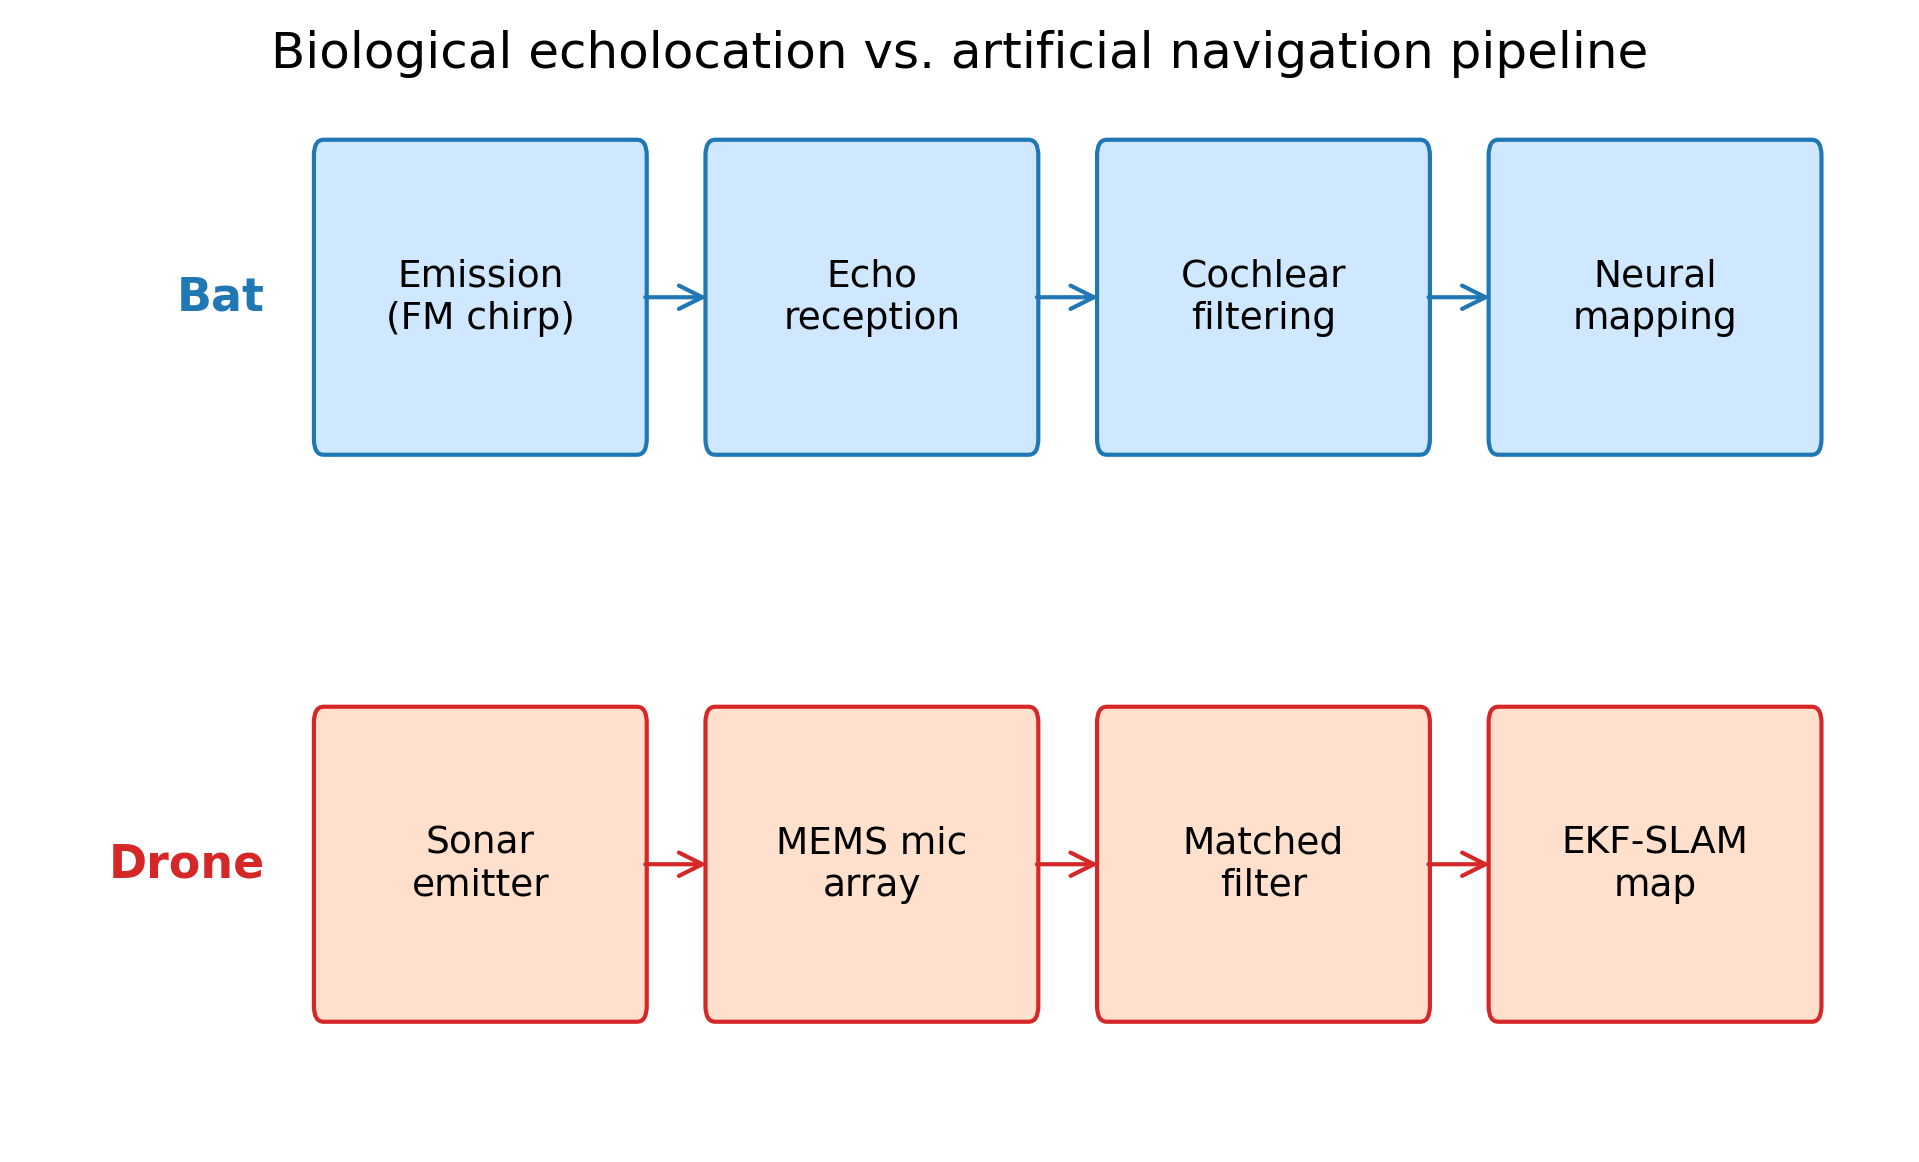
\includegraphics[width=0.95\columnwidth]{figures/fig_algorithm_flowchart.png}
\caption{דיאגרמת זרימה של האלגוריתם המלא לניווט אוטונומי: 8 שלבים בלולאה סגורה בתדר 50 הרץ. (Flowchart of the complete autonomous navigation algorithm: 8 steps in a closed loop at 50 Hz.)}
\label{fig:ch06_algorithm_flow}
\end{figure}

דיאגרמת הזרימה באיור \ref{fig:ch06_algorithm_flow} ממחישה את 8 השלבים של האלגוריתם המלא. החצים המקווקווים מייצגים זרימת מידע בין שלבים, והחצים המלאים מייצגים זרימת בקרה. לולאת המשוב מהשלב השמיני (ניהול משאבים) לשלב הראשון (רכישת חיישנים) מאפשרת התאמה דינמית של תדרי העיבוד בהתאם למצב המערכת. \cite{Thrun2005ProbRobotics} \cite{CrewAIDocs}

\subsection{סיכום}
\label{sec:ch06_summary}

פרק זה הציג את האלגוריתם המלא לניווט אוטונומי, הכולל לולאת ניווט ראשית, תכנון מסלול \en{RRT*} אדפטיבי, זיהוי לולאות סגירה אקוסטיות, מיזוג \en{EKF} אדפטיבי, ניהול משאבים אדפטיבי, והימנעות ממכשולים. האלגוריתם פועל בזמן אמת על פלטפורמת \en{Jetson Orin NX} עם זמן ריצה של 24.1 אלפיות-שנייה למחזור עיבוד מלא. בפרק הבא נציג את ארכיטקטורת המערכת המשולבת וההטמעה בזמן אמת. \cite{Thrun2005ProbRobotics} \cite{CrewAIDocs} \cite{Grisetti2010g2o}

% =============================================================================
% End of Chapter 6
% =============================================================================